\documentclass{beamer}
\usepackage{ices}
\title{Transparent Assessment Framework}
\subtitle{Project outline}
\author{Arni Magnusson\\[0.5ex]Colin Millar}
\date{\green Riga, September 2016}
\begin{document}

\graphicspath{./figs/}

\begin{frame}
  \titlepage\vspace{-7ex}
  
\includegraphics[height=5ex]{logo-1}\hfill
  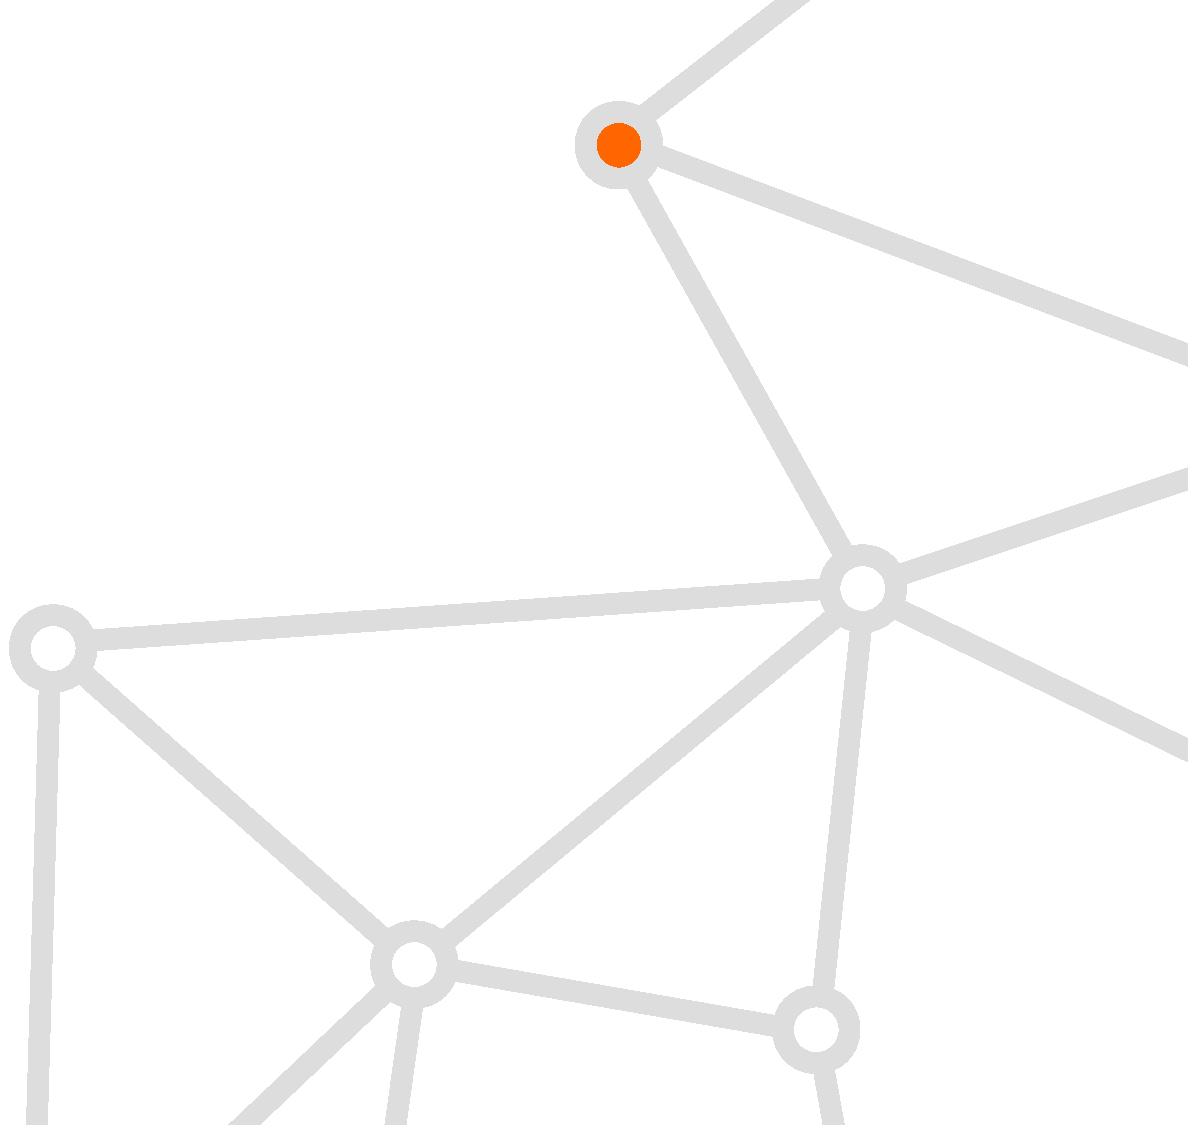
\includegraphics[height=12ex]{logo-2}
\end{frame}

\section{Introduction}
\subsection{Aim}
\begin{frame}{Aim}\it
  To implement a framework to organize {\blue data}, {\blue methods},\\[1ex]
  and {\blue results} used in ICES assessments, so they are\\[1ex]
  easy to {\orange find} and {\orange rerun} later with new data.
\end{frame}

\end{document}
